\scanpage{130}
\figure{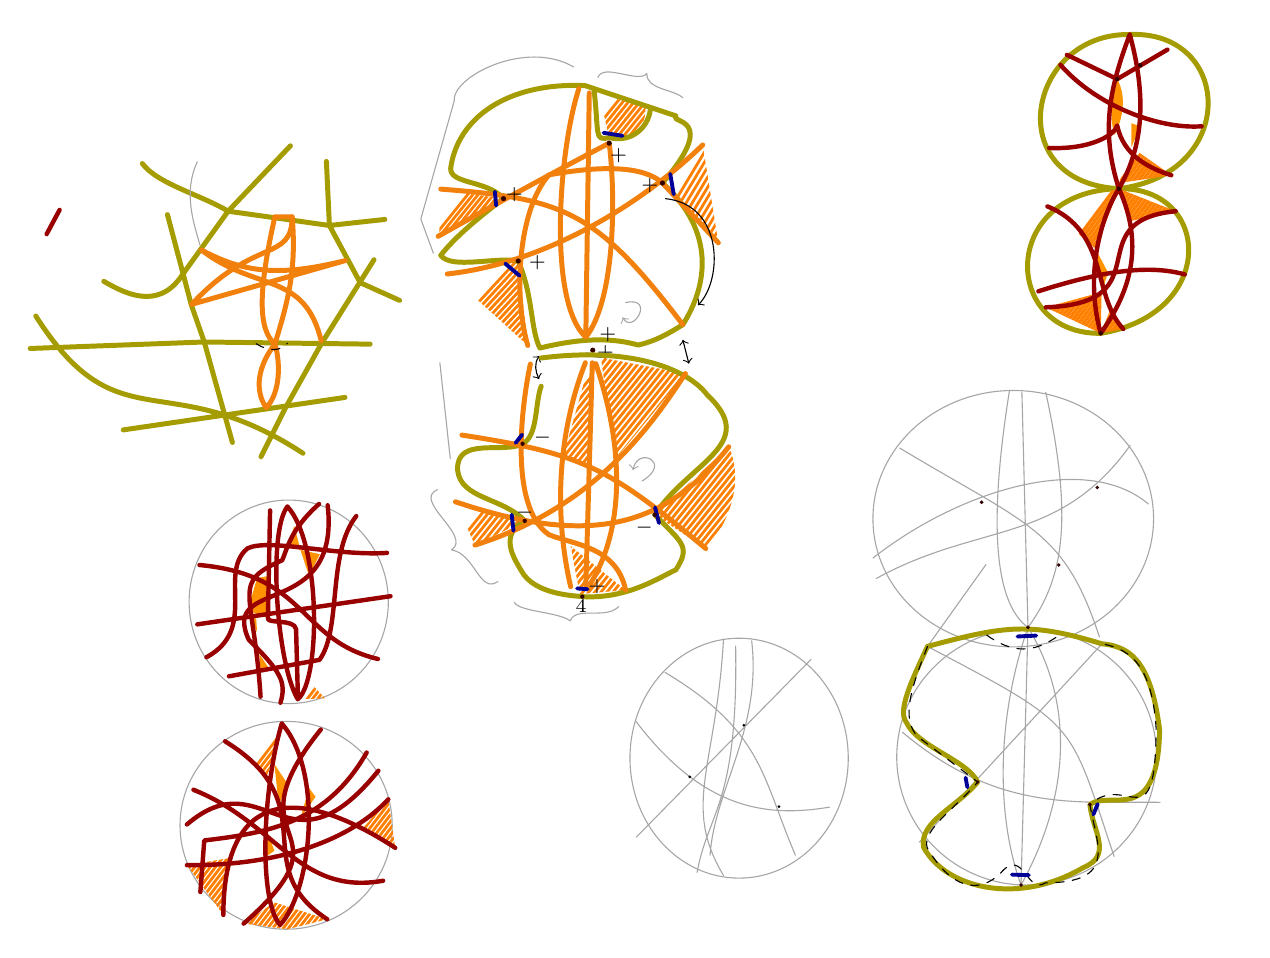
\begin{tikzpicture}[x=.55cm,y=-.55cm,line cap=round,line join=round,g/.style={olive!80!yellow,line width=1.8pt},r/.style={orange!80!brown,line width=1.8pt},w/.style={red!60!black,line width=1.6pt},p/.style={gray!70,thin},b/.style={blue!60!black,line width=1.4pt},every node/.style={font=\scriptsize}]
% E01: upper-left green graph and orange curves.
\draw[g] (3.35,3.68)..controls(3.7,4.15)and(4.7,4.4)..(5.33,4.78)--(6.77,3.27) (5.33,4.78)--(4.26,6.27)..controls(3.7,7.1)and(2.9,6.65)..(2.46,6.4) (3.93,4.86)--(4.48,6.94)--(4.78,7.8)--(5.43,10.12);
\draw[g] (5.33,4.78)--(7.67,5.11)--(8.95,4.97) (7.6,3.63)--(7.67,5.11)--(8.38,6.43)--(9.29,6.84) (8.7,5.9)--(7.49,7.83)--(6.65,9.33)--(6.09,10.45);
\draw[g] (.76,7.95)--(4.78,7.8)--(8.61,7.85) (.89,7.2)..controls(2.8,10.2)and(3.9,8.3)..(7.06,10.37) (2.91,9.83)--(8.03,9.08);
\draw[r] (4.72,5.68)..controls(5.7,6.2)and(6.5,6.3)..(8.04,5.92) (4.49,6.93)--(8.04,5.92) (4.49,6.93)..controls(5.95,5.36)and(6.8,5.96)..(6.81,4.91);
\draw[r] (6.41,4.91)..controls(6.02,6.65)and(6.02,7.5)..(6.41,7.85)..controls(6.73,6.81)and(6.91,6.1)..(6.81,4.91) (6.41,4.91)--(6.81,4.91) (6.41,7.85)..controls(6.02,8.35)and(5.93,8.91)..(6.21,9.32)..controls(6.6,8.9)and(6.5,8.1)..(6.41,7.85) (4.72,5.68)..controls(6,6.66)and(7.08,6.16)..(7.48,7.77);
\draw[p] (4.62,3.64)..controls(4.28,4.36)and(4.55,5.09)..(4.68,5.56);
\draw[w] (1.14,5.31)--(1.44,4.75);
\draw[dashed] (5.98,7.84)..controls(6.27,8.03)and(6.56,8.01)..(6.7,7.83);
% E02: central two-coloured arrangements, hatched boundary regions.
\begin{scope}
\clip (13.9,2.08)--(14.97,2.36)..controls(14.98,2.97)and(14.63,3.06)..(14.13,3.08)--cycle;
\foreach \k in {0,.13,...,2}{\draw[orange,line width=1pt] (13.4+\k,3.4)--(14.6+\k,1.9);}
\end{scope}
\begin{scope}
\clip (10.2,4.28)--(11.69,4.49)--(10.21,5.38)--cycle;
\foreach \k in {0,.12,...,2}{\draw[orange,line width=1pt] (9.9+\k,5.6)--(11.1+\k,4.1);}
\end{scope}
\begin{scope}
\clip (10.4,6.2)--(12.03,5.93)--(12.25,7.88)--cycle;
\foreach \k in {0,.14,...,3}{\draw[orange,line width=1pt] (9.9+\k,8.2)--(12.2+\k,5.7);}
\end{scope}
\begin{scope}
\clip (15.36,4.13)--(16.29,3.25)--(16.65,5.51)--cycle;
\foreach \k in {0,.14,...,3}{\draw[orange,line width=1pt] (14.9+\k,5.8)--(16.4+\k,3.3);}
\end{scope}
\draw[g] (13.57,1.88)..controls(11.75,1.8)and(10.62,2.65)..(10.47,3.79)..controls(10.45,4.16)and(11.32,4.06)..(11.69,4.49)..controls(11.16,4.89)and(10.57,5.37)..(10.24,5.8)..controls(10.48,6.13)and(11.51,5.83)..(12.03,5.93)..controls(12.38,6.75)and(12.31,7.51)..(12.53,7.94)..controls(13.6,7.68)and(14.25,7.72)..(14.8,7.87)..controls(15.2,7.78)and(15.51,7.6)..(15.83,7.4)..controls(16.4,6.5)and(16.6,5.26)..(15.36,4.13)..controls(16.7,2.57)and(15.5,2.76)..(15.67,2.58)--(13.57,1.88);
\draw[g] (13.78,1.97)..controls(13.9,3.04)and(13.78,3.16)..(14.13,3.08)..controls(14.64,3.21)and(15.03,2.85)..(15.08,2.44);
\draw[r] (13.43,1.95)..controls(12.97,3.35)and(12.7,6.86)..(13.59,7.69)..controls(14.26,6.83)and(14.29,4.5)..(14.13,3.21) (13.67,2.05)--(13.59,7.69);
\draw[r] (10.24,4.27)..controls(13.09,4.49)and(13.83,4.77)..(15.83,7.4) (10.18,5.36)..controls(11.75,4.48)and(13.28,3.65)..(14.13,3.21) (10.39,6.23)..controls(12.99,5.94)and(15.22,4.29)..(16.29,3.25);
\draw[r] (12.25,7.88)..controls(11.91,6.72)and(12.03,4.74)..(12.74,3.94)..controls(13.7,3.77)and(14.85,3.67)..(15.36,4.13)--(16.65,5.51);
\draw[p] (13.31,1.45)..controls(12.2,.8)and(10.49,1.68)..(10.55,2.24)--(9.78,4.96)--(10.07,5.75) (13.87,1.69)..controls(14.0,1.35)and(14.81,1.84)..(15.0,1.6)..controls(14.98,1.97)and(15.61,1.96)..(15.83,2.16) (10.22,8.28)--(10.46,10.49);
\draw[->] (15.43,4.49)..controls(16.78,4.63)and(16.75,6.37)..(16.18,6.95);
\draw[p,->] (14.51,6.89)..controls(15.2,6.74)and(14.68,7.64)..(14.44,7.23);
\draw[<->] (15.83,7.75)--(15.97,8.3);
\draw[<->] (12.52,8.12)..controls(12.39,8.3)and(12.43,8.48)..(12.51,8.66);
\foreach \x/\y in {14.35/3.5,11.94/4.39,15.07/4.2,12.47/5.97,14.1/7.62,14.04/8.05}{\node at (\x,\y) {$+$};}
\foreach \x/\y in {14.13/3.21,11.69/4.49,15.36/4.13,12.03/5.93,13.75/7.99}{\fill[red!20!black] (\x,\y) circle (.06);}
\draw[b] (14.0,2.97)--(14.44,3.04) (11.49,4.33)--(11.52,4.65) (15.54,3.92)--(15.62,4.39) (11.73,5.99)--(12.06,6.27) (13.59,8.09)--(13.98,8.12);
\begin{scope}
\clip (12.31,8.31)--(12.13,10.15)--(10.72,9.95)--cycle (13.7,8.2)--(13.07,10.44)--(13.71,10.67)--cycle (13.94,8.16)--(15.89,8.53)--(14.26,10.52)--cycle (15.18,11.79)--(16.89,10.22)..controls(17.32,11.16)and(16.72,12.23)..(16.36,12.57)--cycle (10.58,11.49)--(12.18,11.93)--(11.03,12.49)--cycle (13.24,12.51)--(14.51,13.53)--(13.45,13.62)--cycle;
\foreach \k in {0,.14,...,8}{\draw[orange,line width=1pt] (9.4+\k,14)--(14.6+\k,7.5);}
\end{scope}
\draw[g] (12.56,8.82)..controls(12.41,9.22)and(12.49,9.97)..(12.13,10.15)..controls(11.7,10.39)and(10.59,9.97)..(10.63,10.76)..controls(10.7,11.43)and(11.68,11.39)..(12.18,11.93)..controls(11.56,12.26)and(11.95,12.82)..(12.1,13.08)..controls(12.4,13.65)and(13.39,13.66)..(13.51,13.68)..controls(14.52,13.74)and(15.25,13.26)..(15.67,13.06)..controls(16.03,12.51)and(15.8,12.43)..(15.18,11.79)..controls(15.99,10.57)and(17.61,10.16)..(16.4,9.03)..controls(15.89,8.35)and(14.47,7.92)..(12.56,8.17);
\draw[r] (12.31,8.31)..controls(12.13,9.15)and(11.78,11.59)..(12.74,12.25)..controls(13.3,12.48)and(14.3,12.52)..(14.51,13.53) (13.58,8.28)..controls(13.06,9.6)and(12.78,11.43)..(13.24,13.45) (13.82,8.3)..controls(14.42,10.07)and(14.57,12.08)..(13.62,13.5) (13.74,8.28)--(13.59,13.44);
\draw[r] (10.73,9.95)..controls(13.53,10.38)and(14.12,10.7)..(16.36,12.57) (11.03,12.49)..controls(13.8,11.62)and(15.09,9.74)..(15.89,8.53) (10.58,11.49)..controls(13.59,12.5)and(15.36,12.16)..(16.89,10.22);
\draw[p,->] (14.89,11.01)..controls(15.6,10.58)and(14.79,10.2)..(14.68,10.76);
\draw[p] (10.17,11.21)..controls(9.56,11.45)and(10.98,12.28)..(10.49,12.6)..controls(11.03,12.69)and(11.14,13.63)..(11.56,13.33) (11.94,13.81)..controls(12.04,14.03)and(12.96,14.03)..(13.23,14.24)..controls(13.36,13.89)and(14.05,14.22)..(14.35,13.91);
\draw[b] (12.12,9.94)--(11.97,10.13) (11.88,11.79)--(11.92,12.16) (15.19,11.62)--(15.28,11.98) (13.39,13.49)--(13.63,13.51);
\foreach \x/\y in {12.59/10.02,12.18/11.73,14.94/12.08}{\node at (\x,\y) {$-$};}
\node at (13.85,13.45) {$+$}; \node at (13.48,13.91) {$\unsure{4}$};
\foreach \x/\y in {12.13/10.15,12.18/11.93,15.18/11.79,13.51/13.68}{\fill[red!20!black] (\x,\y) circle (.05);}
% E03: two small upper-right circles.
\fill[orange!85!yellow] (25.86,1.73)..controls(25.72,2.15)and(25.68,2.65)..(25.8,3.02)..controls(26.01,2.61)and(26.07,2.1)..(25.86,1.73);
\fill[orange!85!yellow] (26.19,2.75)--(26.39,2.82)--(26.19,3.3)--cycle (25.36,5.65)--(25.65,6.2)--(25.5,6.65)--cycle;

\draw[g] (26.15,.7)..controls(28.53,.6)and(28.68,3.91)..(25.9,4.26)..controls(23.15,4.12)and(23.77,.67)..(26.15,.7);
\draw[g] (25.9,4.26)..controls(28.05,4.23)and(28.18,7.15)..(25.48,7.6)..controls(23.19,7.63)and(23.13,4.32)..(25.9,4.26);
\begin{scope}
\clip (24.7,1.17)--(25.86,1.73)--(26.09,.77)--cycle (26.29,.78)--(26.39,1.41)--(27.02,1.05)--cycle (24.29,3.32)--(25.8,3.02)--(25.88,4.13)--cycle (25.9,4.13)--(26.19,3.3)--(27.11,3.95)--cycle (24.25,4.67)--(25.9,4.26)--(25.36,5.65)--cycle (25.9,4.26)--(26.16,5.01)--(27.21,4.78)--cycle (24.21,7.0)--(25.5,6.65)--(25.48,7.6)--cycle (25.48,7.6)--(25.72,7.0)--(26.0,7.5)--cycle;
\foreach \k in {0,.1,...,5}{\draw[orange,line width=1.2pt] (23+\k,8)--(29+\k,0);}
\end{scope}
\draw[w] (26.15,.7)..controls(26.59,2.3)and(26.4,3.39)..(25.9,4.26)..controls(25.46,2.9)and(25.7,1.9)..(26.15,.7) (24.7,1.17)--(25.86,1.73)--(27.02,1.05) (24.55,1.4)..controls(25.38,2.35)and(26.82,2.89)..(27.81,2.82) (24.29,3.32)..controls(25.25,3.36)and(25.81,3.02)..(25.86,2.8)..controls(26.0,3.49)and(26.59,3.79)..(27.11,3.95);
\draw[w] (25.9,4.26)..controls(26.54,5.67)and(26.08,6.75)..(25.48,7.6)..controls(25.07,6.12)and(25.56,4.78)..(25.9,4.26) (24.25,4.67)..controls(25.67,5.25)and(25.28,6.73)..(26.0,7.5) (24.21,7.0)..controls(26.95,6.9)and(24.9,5.01)..(27.21,4.78) (24.04,6.63)..controls(25.6,6.13)and(26.63,6.02)..(27.42,6.24);
\foreach \x/\y in {25.86/1.73,26.39/1.41,25.9/4.26,25.48/7.6}{\fill[red!20!black] (\x,\y) circle (.05);}
% E04 and E05: two lower-left red arrangements.
\fill[orange!85!yellow] (6.86,12.05)--(7.0,12.6)--(6.7,12.5)--cycle (7.0,12.6)--(7.45,12.7)--(7.2,13.2)--cycle (6.0,13.25)--(6.28,13.2)--(6.25,14.17)--(5.78,14.0)--cycle (5.78,14.0)--(6.0,14.5)--(5.98,14.2)--cycle (6.05,15.0)--(6.25,15.3)--(6.08,15.4)--cycle (6.4,17.55)--(6.7,18.0)--(6.5,18.5)--cycle (7.2,18.1)--(7.35,18.3)--(7.0,18.8)--cycle (6.2,19.0)--(6.4,19.55)--(6.18,19.7)--cycle;

\draw[p] (6.73,13.80) ellipse (2.3 and 2.35);
\draw[p] (6.67,18.96) ellipse (2.45 and 2.4);
\begin{scope}
\clip (7.92,12.68)--(8.29,11.82)--(9.0,12.67)--cycle (4.62,14.32)--(5.46,14.22)--(4.83,15.08)--cycle (5.35,15.52)--(6.08,15.38)--(6.08,15.99)--cycle (6.91,16.05)--(7.16,15.6)--(7.57,16.03)--cycle (5.26,17.02)--(6.57,16.61)--(6.24,17.83)--cycle (4.53,18.14)--(4.38,18.94)--(5.16,18.46)--cycle (8.44,19.03)--(9.03,18.36)--(9.19,19.48)--cycle (4.38,19.88)--(5.34,19.72)--(5.22,21.03)--cycle (5.69,21.23)--(6.4,20.74)--(7.62,21.13)--(6.7,21.36)--cycle;
\foreach \k in {0,.12,...,6}{\draw[orange,line width=1pt] (3+\k,21.5)--(11+\k,11);}
\end{scope}
\draw[w] (6.3,11.69)--(6.25,14.17)..controls(6.2,14.32)and(6.86,14.18)..(6.9,14.43)--(6.94,15.91) (6.7,11.6)..controls(7.48,12.45)and(7.47,15.61)..(6.94,16.05)..controls(6.45,15.23)and(6.24,12.19)..(6.7,11.6) (7.63,11.57)..controls(7.93,14.26)and(5.12,13.19)..(5.81,14.68)..controls(6.56,15.42)and(6.68,15.66)..(6.54,16.13);
\draw[w] (7.43,11.54)..controls(6.77,12.13)and(6.7,12.56)..(6.58,12.84)..controls(5.39,13.37)and(5.92,13.49)..(6.08,15.99) (8.29,11.82)..controls(7.61,12.69)and(7.96,14.43)..(7.44,15.14)--(5.35,15.52) (4.62,14.32)--(9.08,13.67) (4.83,15.08)..controls(6.03,14.43)and(5.09,13.16)..(5.77,12.57)..controls(6.25,12.32)and(7.82,12.75)..(9.0,12.67) (4.67,12.95)..controls(7.18,13.18)and(6.95,14.68)..(8.79,15.12);
\draw[w] (6.57,16.61)..controls(6.13,18.1)and(6.02,20.67)..(6.53,21.26)..controls(7.24,20.5)and(7.56,17.76)..(6.57,16.61) (7.47,16.75)..controls(5.25,19.5)and(8.33,18.9)..(5.69,21.23) (5.26,17.02)..controls(7.63,18.48)and(5.72,19.89)..(7.62,21.13) (4.53,18.14)..controls(6.45,18.9)and(6.96,20.59)..(8.91,20.24) (4.38,18.94)..controls(6.18,17.4)and(6.7,20.3)..(8.8,17.7) (4.38,19.88)..controls(6.63,19.9)and(8.22,19.24)..(9.03,18.36) (4.69,20.5)--(4.78,19.31)..controls(6.3,19.13)and(7.61,18.89)..(8.53,17.28) (5.22,21.03)..controls(5.23,18.14)and(6.91,18.0)..(9.19,19.48);
% E06: lower-centre pencil circle.
\draw[p] (17.13,17.41) ellipse (2.52 and 2.77);
\draw[p] (16.77,14.66)..controls(16.6,17.64)and(15.8,18.49)..(16.77,20.12) (17.05,14.82)..controls(17.11,18.51)and(16.41,18.64)..(16.16,20.05) (17.42,14.7)..controls(17.66,16.74)and(16.56,18.13)..(16.46,19.65) (15.42,15.43)..controls(17.68,16.78)and(17.66,17.86)..(18.43,19.65) (14.74,16.55)..controls(16.28,18.58)and(17.74,18.79)..(19.22,18.54) (14.76,19.23)--(18.79,15.13);
\foreach \x/\y in {15.99/17.84,17.24/16.65,18.05/18.53}{\fill (\x,\y) circle (.035);}
% E07: right-hand pencil pair and irregular green boundary.
\draw[p] (23.46,11.88) ellipse (3.24 and 2.96);
\draw[p] (23.77,17.38) ellipse (3.0 and 2.96);
\draw[p] (23.37,8.94)..controls(22.94,11.64)and(22.94,13.77)..(23.8,14.39)..controls(24.66,13.23)and(24.83,11.8)..(24.21,8.96) (23.66,8.96)--(23.8,14.39) (20.84,10.25)..controls(23.81,12.04)and(24.63,12.11)..(25.45,14.61) (20.22,12.79)..controls(22.15,11.27)and(25.1,10.3)..(26.58,11.54) (20.3,13.26)..controls(22.68,11.95)and(24.5,12.5)..(26.16,10.19) (21.48,14.83)--(22.83,12.94);
\draw[p] (21.48,14.83)..controls(25.03,16.7)and(24.73,16.54)..(25.79,19.68) (20.9,16.81)..controls(23.14,18.69)and(24.96,18.4)..(26.85,18.43) (23.8,14.39)..controls(23.06,16.53)and(23.07,18.77)..(23.64,20.34)..controls(24.79,18.25)and(24.86,16.12)..(23.8,14.39) (23.8,14.39)--(23.64,20.34) (21.29,19.35)--(25.51,14.77);
\draw[g] (21.48,14.83)..controls(21.11,15.63)and(20.78,16.32)..(20.99,16.58)..controls(21.25,17.15)and(22.39,17.45)..(22.64,17.96)..controls(22.15,18.55)and(21.28,18.88)..(21.39,19.47)..controls(21.93,20.45)and(23.61,20.8)..(25.07,19.94)..controls(25.78,19.65)and(25.29,19.1)..(25.23,18.48)..controls(25.72,18.13)and(26.8,19.01)..(26.84,16.76)..controls(26.66,15.35)and(26.27,14.83)..(25.51,14.77)..controls(23.85,14.27)and(23.3,14.34)..(21.48,14.83);
\draw[dashed] (21.48,14.83)..controls(21.11,15.78)and(20.86,16.48)..(21.25,16.91)--(22.64,17.96)..controls(22.15,18.55)and(21.35,19.06)..(21.47,19.47)..controls(22.0,20.4)and(22.65,20.59)..(23.18,20.05)..controls(23.69,19.46)and(23.78,20.58)..(24.2,20.29)..controls(25.88,20.28)and(25.39,19.43)..(25.23,18.48)..controls(26.09,17.7)and(26.74,19.4)..(26.76,16.73)..controls(26.67,15.38)and(26.25,14.9)..(25.51,14.77) (22.85,14.57)..controls(23.45,15.0)and(23.94,14.99)..(24.52,14.57);
\draw[b] (23.56,14.6)--(23.99,14.58) (22.36,17.86)--(22.4,18.08) (25.41,18.47)--(25.31,18.71) (23.43,20.1)--(23.82,20.11);
\foreach \x/\y in {22.73/11.5,25.4/11.16,24.51/12.95,23.8/14.39,22.64/17.96,25.23/18.48,23.64/20.34}{\fill[red!20!black] (\x,\y) circle (.045);}
\end{tikzpicture}}
\margin{\mspage{129}}
